%% Template for MLP Coursework 1 / 16 October 2017 

%% Based on  LaTeX template for ICML 2017 - example_paper.tex at 
%%  https://2017.icml.cc/Conferences/2017/StyleAuthorInstructions

\documentclass{article}

\usepackage[T1]{fontenc}
\usepackage{amssymb,amsmath}
\usepackage{txfonts}
\usepackage{microtype}

% For figures
\usepackage{graphicx}
\usepackage{subfigure} 

% For citations
\usepackage{natbib}

% For algorithms
\usepackage{algorithm}
\usepackage{algorithmic}

% the hyperref package is used to produce hyperlinks in the
% resulting PDF.  If this breaks your system, please commend out the
% following usepackage line and replace \usepackage{mlp2017} with
% \usepackage[nohyperref]{mlp2017} below.
\usepackage{hyperref}
\usepackage{url}
\urlstyle{same}

% Packages hyperref and algorithmic misbehave sometimes.  We can fix
% this with the following command.
\newcommand{\theHalgorithm}{\arabic{algorithm}}


% Set up MLP coursework style (based on ICML style)
\usepackage{mlp2017}
\mlptitlerunning{MLP Coursework 1 (\studentNumber)}
\bibliographystyle{icml2017}


\DeclareMathOperator{\softmax}{softmax}
\DeclareMathOperator{\sigmoid}{sigmoid}
\DeclareMathOperator{\sgn}{sgn}
\DeclareMathOperator{\relu}{relu}
\DeclareMathOperator{\lrelu}{lrelu}
\DeclareMathOperator{\elu}{elu}
\DeclareMathOperator{\selu}{selu}
\DeclareMathOperator{\maxout}{maxout}

%% You probably do not need to change anything above this comment

%% REPLACE this with your student number
\def\studentNumber{s1754321}

\begin{document} 

\twocolumn[
\mlptitle{MLP Coursework 1: Activation Functions}

\centerline{\studentNumber}

\vskip 7mm
]

\begin{abstract} 
The abstract should be 100--200 words long,  providing a concise summary of the contents of your report.
\end{abstract} 

\section{Introduction}
\label{sec:intro}
This document provides a template for the MLP coursework 1 report.  In particular, it structures the document into five sections  (plus an abstract and the references) -- you should keep to this structure for your report.  If you want to use subsections within a section that is fine, but please do not use any deeper structuring.  In this template the text in each section will include an outline of what you should include in each section, along with some practical LaTeX examples (for example figures, tables, algorithms).  Your document should be no longer than \textbf{six pages},  with an additional page allowed for references.

The introduction should place your work in context, giving the overall motivation for the work, and clearly outlining the research questions you have explored -- in this case comparison of the behaviour of the different activation functions,  experimental investigation of the impact of the depth of the network with respect to accuracy, and experimental investigation of different approaches to weight initialisation.  This section should also include a concise description of the MNIST task and  data -- be precise: for example state the size of the training and validation sets.


\section{Activation functions}
\label{sec:actfn}
This section should cover the theoretical methodology -- in this case you should present the four activation functions: ReLU, Leaky ReLU, ELU, and SELU.  I didn't do it in this document, but the first time you use an acronym you should say what it stands for, for example Restricted Linear Unit (ReLU).  You should use equations to concisely describe each activation function.  For example, ReLU: 
\begin{equation}
  \relu(x) = \max(0, x) ,
\end{equation} 
which has the gradient:
\begin{equation}
  \frac{d}{dx} \relu(x) =
     \begin{cases} 
      0      & \quad \text{if } x \leq  0 \\
      1       & \quad \text{if } x > 0 .
    \end{cases} 
\end{equation}
The \LaTeX for the derivatives is slightly more complicated.  We provided definitions near the top of the file (the part before \verb+\begin{document}+) for \verb+\relu+, \verb+\lrelu+, \verb+\elu+, and \verb+\selu+.  There is no need to discuss the unit tests for these activation functions in this report.

It is probably not needed in this report, but if you would like to include an algorithm in your report, please use the \verb+algorithm+ and \verb+algorithmic+ environments to format pseudocode (for instance, Algorithm~\ref{alg:example}). These require the corresponding style files, \verb+algorithm.sty+ and \verb+algorithmic.sty+ which are supplied with this package. 

\begin{algorithm}[ht]
\begin{algorithmic}
   \STATE {\bfseries Input:} data $x_i$, size $m$
   \REPEAT
   \STATE Initialize $noChange = true$.
   \FOR{$i=1$ {\bfseries to} $m-1$}
   \IF{$x_i > x_{i+1}$} 
   \STATE Swap $x_i$ and $x_{i+1}$
   \STATE $noChange = false$
   \ENDIF
   \ENDFOR
   \UNTIL{$noChange$ is $true$}
\end{algorithmic}
  \caption{Bubble Sort}
  \label{alg:example}
\end{algorithm}

\section{Experimental comparison of activation functions}
\label{sec:actexpts}
In this section you should present the results and discussion of your experiments comparing networks using the different activation functions on the MNIST task.  As explained in the coursework document, you should use 2 hidden layers with 100 hidden units per layer for these experiments.  You can compare the learning curves (error vs epoch) for training and/or validation, and the validation set accuracies. 

Your experimental sections should include graphs (for instance, figure~\ref{fig:sample-graph}) and/or tables (for instance, table~\ref{tab:sample-table})\footnote{These examples were taken from the ICML template paper.}, using the \verb+figure+ and \verb+table+ environments, in which you use \verb+\includegraphics+ to include an image (pdf, png, or jpg formats).  Please export graphs as 
\href{https://en.wikipedia.org/wiki/Vector_graphics}{vector graphics}
rather than \href{https://en.wikipedia.org/wiki/Raster_graphics}{raster
files} as this will make sure all detail in the plot is visible.
Matplotlib supports saving high quality figures in a wide range of
common image formats using the
\href{http://matplotlib.org/api/pyplot_api.html\#matplotlib.pyplot.savefig}{\texttt{savefig}}
function. \textbf{You should use \texttt{savefig} rather than copying
the screen-resolution raster images outputted in the notebook.} An
example of using \texttt{savefig} to save a figure as a PDF file (which
can be included as graphics in a \LaTeX document is given in the coursework document.

If you need a figure or table to stretch across two columns use the \verb+figure*+ or \verb+table*+ environment instead of the \verb+figure+ or \verb+table+ environment.  Use the \verb+subfigure+ environment if you want to include multiple graphics in a single figure.

\begin{figure}[tb]
\vskip 5mm
\begin{center}
\centerline{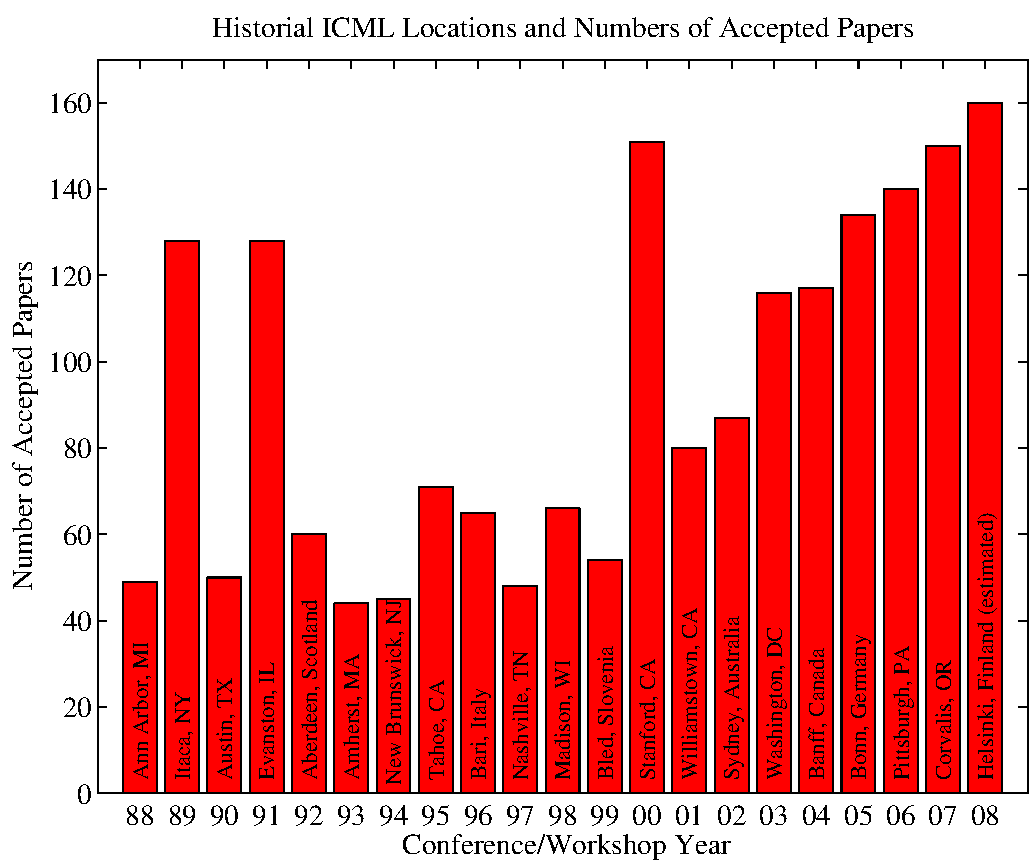
\includegraphics[width=\columnwidth]{icml_numpapers}}
\caption{Historical locations and number of accepted papers for International
  Machine Learning Conferences (ICML 1993 -- ICML 2008) and
  International Workshops on Machine Learning (ML 1988 -- ML
  1992). At the time this figure was produced, the number of
  accepted papers for ICML 2008 was unknown and instead estimated.}
\label{fig:sample-graph}
\end{center}
\vskip -5mm
\end{figure} 

\begin{table}[tb]
\vskip 3mm
\begin{center}
\begin{small}
\begin{sc}
\begin{tabular}{lcccr}
\hline
\abovespace\belowspace
Data set & Naive & Flexible & Better? \\
\hline
\abovespace
Breast    & 95.9$\pm$ 0.2& 96.7$\pm$ 0.2& $\surd$ \\
Cleveland & 83.3$\pm$ 0.6& 80.0$\pm$ 0.6& $\times$\\
Glass2    & 61.9$\pm$ 1.4& 83.8$\pm$ 0.7& $\surd$ \\
Credit    & 74.8$\pm$ 0.5& 78.3$\pm$ 0.6&         \\
Horse     & 73.3$\pm$ 0.9& 69.7$\pm$ 1.0& $\times$\\
Meta      & 67.1$\pm$ 0.6& 76.5$\pm$ 0.5& $\surd$ \\
Pima      & 75.1$\pm$ 0.6& 73.9$\pm$ 0.5&         \\
\belowspace
Vehicle   & 44.9$\pm$ 0.6& 61.5$\pm$ 0.4& $\surd$ \\
\hline
\end{tabular}
\end{sc}
\end{small}
\caption{Classification accuracies for naive Bayes and flexible 
Bayes on various data sets.}
\label{tab:sample-table}
\end{center}
\vskip -3mm
\end{table}

\section{Deep neural network experiments}
\label{sec:dnnexpts}
This section should report on your experiments on deeper networks for MNIST.  The two sets of experiments are to explore the impact of the depth of the network (number of hidden layers), and a comparison of different approaches to weight initialisation.

In this section, and in the previous section, you should present your experimental results clearly and concisely, followed by an interpretation and discussion of results. You need to present your results in a way that makes it easy for a reader to understand what they mean. You should facilitate comparisons either using graphs with multiple curves or (if appropriate, e.g. for accuracies) a results table. You need to avoid having too many figures, poorly labelled graphs, and graphs which should be comparable but which use different axis scales. A good presentation will enable the reader to compare trends in the same graph -- each graph should summarise the results relating to a particular research (sub)question.

Your discussion should interpret the results, both in terms of summarising the outcomes of a particular experiment, and attempting to relate to the underlying models. A good report would have some analysis, resulting in an understanding of why particular results are observed, perhaps with reference to the literature. Use bibtex to organise your references -- in this case the references are in the file \verb+example-refs.bib+.  Here is a an example reference \citep{langley00}.  




\section{Conclusions}
\label{sec:concl}
You should draw conclusions from the experiments, related to the research questions outlined in the introduction (section~\ref{sec:intro}). You should state the conclusions clearly and concisely. It is good if the conclusion from one experiment influenced what you did in later experiments -- your aim is to learn from your experiments. Extra credit if you relate your findings to what has been reported in the literature.

A good conclusions section would also include a further work discussion, building on work done so far, and referencing the literature where appropriate.

\bibliography{example-refs}

\end{document} 


% This document was modified from the file originally made available by
% Pat Langley and Andrea Danyluk for ICML-2K. This version was
% created by Lise Getoor and Tobias Scheffer, it was slightly modified  
% from the 2010 version by Thorsten Joachims & Johannes Fuernkranz, 
% slightly modified from the 2009 version by Kiri Wagstaff and 
% Sam Roweis's 2008 version, which is slightly modified from 
% Prasad Tadepalli's 2007 version which is a lightly 
% changed version of the previous year's version by Andrew Moore, 
% which was in turn edited from those of Kristian Kersting and 
% Codrina Lauth. Alex Smola contributed to the algorithmic style files.  
